\pagenumbering{arabic}

\chapter{Introduction} \label{introduction}

\paragraph{}
This document is the Software Requirements Specification (SRS) \cite{iso29148} for the open-source project Koster Seafloor Observatory (KSO). KSO is a modular, open-source software platform developed to support marine ecological research through the analysis of underwater video data. It integrates citizen science, machine learning, and high-performance computing to enable large-scale annotation, classification, and interpretation of subsea imagery. The system includes tools for data management, species identification through crowdsourced annotations, and automated biological object detection, facilitating reproducible and scalable biodiversity monitoring in marine environments.
\section{Purpose of the System }
The \textbf{Koster Seafloor Observatory (KSO)} is an \textbf{open-source} initiative designed to facilitate the efficient management, annotation, and analysis of large volumes of underwater footage for \textbf{marine ecological research}. The system integrates \textbf{citizen science and machine learning} to enhance the identification and monitoring of marine biodiversity. KSO enables researchers to collect, process, and analyze data from underwater recordings, particularly those captured in Sweden’s \textbf{Kosterhavets National Park}. By leveraging \textbf{public participation} and \textbf{high-performance computing}, the system enhances the efficiency and scalability of marine biodiversity assessments.

KSO's purpose includes:
\begin{itemize}
    \item \textbf{Data Management}: Storing and archiving subsea footage for research purposes.
    \item \textbf{Citizen Science Participation}: Enabling volunteers to annotate video clips to support marine species identification.
    \item \textbf{Machine Learning Integration}: Using citizen-provided classifications to train AI models for automated species recognition.
    \item \textbf{Ecological Research Support}: Providing scientists with analytical tools to monitor marine biodiversity and assess environmental changes over time.
\end{itemize}

By \textbf{combining open-source tools, citizen science, and AI-based automation}, KSO aims to enhance the accessibility and accuracy of marine biodiversity research.


\section{Scope}

The \textbf{Koster Seafloor Observatory (KSO)} is a \textbf{modular software system} that focuses on the collection, classification, and automated analysis of underwater imagery. Its primary application is within \textbf{marine ecological research}, specifically for monitoring \textbf{cold-water coral reefs} and other benthic habitats in the \textbf{Kosterhavets National Park}.

The system is structured into three core modules:
\begin{enumerate}
    \item \textbf{Data Management Module} – Facilitates the storage and processing of large-scale underwater video footage, ensuring \textbf{long-term archiving} and accessibility for researchers.
    \item \textbf{Citizen Science Module} – Engages volunteers to classify and annotate marine species using a \textbf{web-based platform}, enhancing data collection efficiency.
    \item \textbf{Machine Learning \& High-Performance Computing Module} – Utilizes annotated data to train and deploy \textbf{machine learning models} for \textbf{automated species identification} and habitat mapping.
\end{enumerate}

The \textbf{scope} of KSO extends to:
\begin{itemize}
    \item Processing \textbf{high-definition} underwater video footage collected from \textbf{remotely operated vehicles (ROVs)}.
    \item Hosting \textbf{citizen science campaigns} for \textbf{species annotation} via platforms like \textbf{Zooniverse}.
    \item Training and deploying \textbf{AI-based detection models} to classify marine species and habitats.
    \item Providing an \textbf{API-based interface} for researchers to interact with trained models and analyze ecological data.
\end{itemize}

The system is intended for use by \textbf{marine biologists, ecologists, AI researchers, and citizen scientists} interested in marine conservation and biodiversity monitoring. Future expansions may include \textbf{support for additional marine ecosystems}, \textbf{enhanced deep-learning models}, and \textbf{improved real-time processing capabilities}.

\section{System Overview}


\subsection{System Perspective}

The \textbf{Koster Seafloor Observatory (KSO)} serves as a central hub for managing, processing, and analyzing subsea video data for marine ecological research. It facilitates interactions between \textbf{citizen scientists, researchers, storage servers, machine learning models, and biodiversity databases} to streamline underwater biodiversity monitoring.

\begin{figure}[ht]
    \centering
    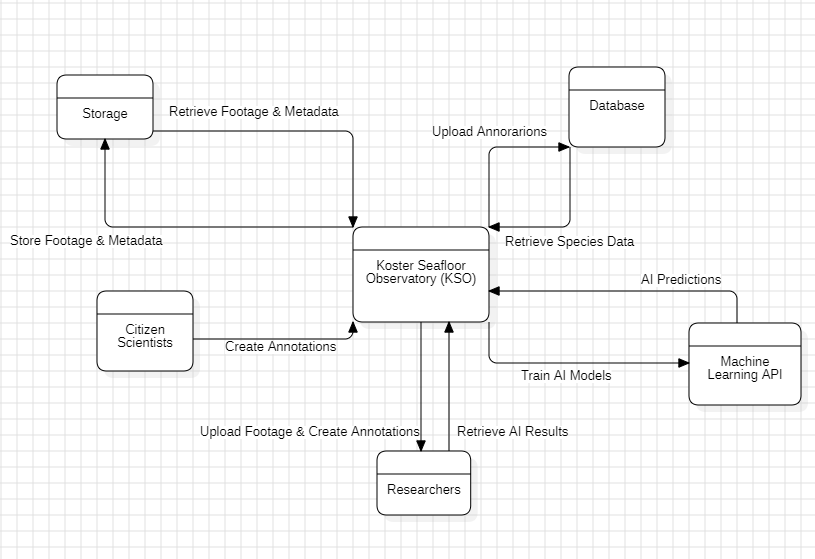
\includegraphics[width=.9 \textwidth]{Figures/System Context Diagram.png}
    \caption{System Context Diagram \label{Fig:System Context Diagram}}
\end{figure}

The system operates through a series of key interactions:
\begin{itemize}
    \item \textbf{Citizen scientists} contribute by creating annotations of marine species in underwater footage.
    \item \textbf{Researchers} upload new footage and contribute to annotation efforts.
    \item \textbf{KSO} stores and retrieves footage and metadata from a \textbf{storage server} for efficient data management.
    \item \textbf{Machine learning models} are trained using annotations from citizen scientists, and the trained models provide \textbf{AI-based species predictions} to researchers.
    \item \textbf{Biodiversity databases} receive and share species data to enhance broader ecological studies.
\end{itemize}

By integrating \textbf{open-source tools, participatory science, and machine learning}, the KSO enables scalable and efficient marine biodiversity monitoring. \textbf{Technical implementation details} of these interactions are further explored in \textbf{Section 3}.

\subsubsection{System Interfaces}
The KSO system interfaces with several external and internal components:
\begin{itemize}
    \item \textbf{Citizen Science Platform (Zooniverse API)} – Facilitates seamless integration of user annotations into KSO's database.
    \item \textbf{Machine Learning API (FastAPI)} – Provides AI-powered species classification by processing annotated video footage.
    \item \textbf{Storage and Database Services} – Manages metadata, classification data, and video footage in SQL-based storage.
    \item \textbf{Visualization Toolkit} – Offers researchers a graphical interface for exploring and validating ecological data.
\end{itemize}

\subsubsection{User Interfaces}
KSO provides multiple user interaction points:
\begin{itemize}
    \item \textbf{Web-Based Citizen Science Platform}: A Zooniverse-hosted interface that enables volunteers to annotate species in video clips and images.
    \item \textbf{Researcher Dashboard}: A Streamlit-based front-end for uploading footage, analyzing results, and fine-tuning machine learning model parameters.
    \item \textbf{API-Driven Access}: Advanced users can interact with KSO’s trained models and datasets through programmatic API requests.
\end{itemize}

Future improvements may include an enhanced UI with interactive real-time video annotation tools and improved accessibility for mobile platforms.

\subsubsection{Hardware Interfaces}
The Koster Seafloor Observatory (KSO) operates on a distributed computing architecture that integrates high-performance storage and processing hardware. The key hardware components include:

\begin{itemize}
    \item \textbf{High-Performance Computing (HPC) Server}: Utilized for machine learning training and video processing, equipped with:
    \begin{itemize}
        \item \textbf{GPU}: NVIDIA GTX 2080Ti for accelerated deep learning inference.
        \item \textbf{CPU}: Intel Core i9-9900 (16 cores, 3.10 GHz).
        \item \textbf{RAM}: 2GB DDR4 memory.
    \end{itemize}
    \item \textbf{Long-Term Storage (Cold Storage)}: Archive for large video datasets, hosted on university research servers.
    \item \textbf{Short-Term Storage (Hot Storage)}: Linux-based server hosting frequently accessed video files for annotation and model training.
    \item \textbf{Remote Operated Vehicles (ROVs)}: Used for collecting underwater footage; hardware specifications may vary based on deployment.
\end{itemize}

\subsubsection{Software Interfaces}

KSO integrates various software components for data processing, annotation, and machine learning. The key software interfaces include:

\begin{itemize}
    \item \textbf{Operating System}: Linux-based environment for high-performance computing.
    \item \textbf{Machine Learning Frameworks}: YOLOv3 for training species identification models.
    \item \textbf{Database}: SQLite for metadata storage and annotation tracking.
    \item \textbf{Web Interface}: Developed using Streamlit for researcher access.
    \item \textbf{API Services}:
    \begin{itemize}
        \item \textbf{Zooniverse API}: Handles citizen scientist annotations.
        \item \textbf{FastAPI}: Facilitates AI model access for automated classification.
        \item \textbf{Data Visualization API}: Provides mapping and graphical representation of species occurrences.
    \end{itemize}
\end{itemize}

\subsubsection{Communication Interfaces}

The Koster Seafloor Observatory (KSO) utilizes APIs (FastAPI) for seamless data exchange, a Streamlit web interface for user-friendly model interaction, and Zooniverse for engaging citizen scientists. These interfaces enable efficient communication between data storage, analysis modules, and users, ensuring smooth collaboration in marine ecological research.

\subsubsection{Memory Constraints}

The Koster Seafloor Observatory (KSO) project deals with massive high-resolution video datasets, requiring efficient memory management for storage, processing, and analysis. 

Storage constraints arise due to the need to archive large volumes of footage while maintaining a subset in hot storage for active processing. Processing constraints include handling high-resolution video files, extracting frames, and aggregating citizen science annotations, all of which require significant RAM and computational power.

A major limitation is the \textbf{2GB DDR4 RAM}, which is \textbf{insufficient for such a large-scale project}. Training deep learning models, processing high-resolution imagery, and running real-time inference on large datasets demand significantly more memory. Machine learning models like YOLOv3 require substantial computational resources, and 2GB RAM severely limits performance, causing bottlenecks in data loading, training speed, and inference accuracy.

API and user interaction constraints further strain memory, as handling multiple concurrent requests and visualizing large datasets requires efficient resource allocation. To address these issues, optimization strategies such as data compression, incremental loading, and upgrading to a higher RAM capacity are essential. A more powerful GPU with at least \textbf{16GB RAM} is recommended to handle the computational demands of large-scale marine data analysis.


\subsubsection{Operations}

\textbf{System Operations:}
\begin{itemize}
    \item Store and manage subsea video data
    \item Process and archive underwater recordings
    \item Extract frames from video clips
    \item Manage metadata in a structured database
    \item Aggregate annotations from citizen scientists
    \item Train and validate machine learning models
    \item Run object detection on new video data
    \item Provide API access for model predictions
    \item Display machine learning model results
    \item Authenticate and manage user access
\end{itemize}
\textbf{User Operations:}
\begin{itemize}
    \item Upload underwater footage for analysis
    \item Annotate video clips via citizen science platform
    \item View and edit species classifications
    \item Access machine learning predictions via API
    \item Adjust confidence thresholds for model output
    \item Visualize spatial distribution of marine species
    \item Download annotated datasets for research
    \item Log in to web application for data access
    \item Customize processing parameters for analysis
\end{itemize}

\subsection{System Functions}

System functions are defined in Table \ref{tab:kso_system_functions}

\begin{table}[H]
    \centering
    \footnotesize
    \renewcommand{\arraystretch}{1.2}
    \begin{tabular}{|l|p{10cm}|}
        \hline
        \textbf{Function} & \textbf{Summary} \\
        \hline
        \textbf{Data Storage \& Retrieval} & Provides long-term (cold storage) and short-term (hot storage) data management for efficient archiving and retrieval of subsea footage. \\
        \hline
        \textbf{Metadata Management} & Organizes movie metadata in a structured SQLite database following Darwin Core (DwC) standards. \\
        \hline
        \textbf{Data Processing} & Splits long subsea movies into manageable clips and processes annotations for further analysis. \\
        \hline
        \textbf{User Engagement} & Involves citizen scientists in annotating subsea videos through an intuitive web interface on Zooniverse. \\
        \hline
        \textbf{Species Classification} & Enables users to classify species present in subsea footage and report their observations. \\
        \hline
        \textbf{Object Localization} & Allows citizen scientists to mark specific species by drawing bounding boxes on still images. \\
        \hline
        \textbf{Data Aggregation} & Ensures annotation reliability by applying agreement thresholds before using them in machine learning. \\
        \hline
        \textbf{Model Training \& Testing} & Uses labeled datasets from citizen scientists to train and validate deep learning models (e.g., YOLOv3). \\
        \hline
        \textbf{Automated Detection} & Deploys trained models to detect and classify species in new subsea footage. \\
        \hline
        \textbf{Hyperparameter Tuning} & Allows users to adjust detection thresholds (confidence, overlap) to refine model performance. \\
        \hline
        \textbf{API Access} & Provides an API for researchers to integrate trained models into their own workflows. \\
        \hline
        \textbf{Data Visualization} & Generates spatial distribution maps of detected species to support ecological research. \\
        \hline
    \end{tabular}
    \caption{System Functions of Koster Seafloor Observatory (KSO)}
    \label{tab:kso_system_functions}
\end{table}

\subsection{Stakeholder Characteristics}

There are two main users of the Koster Seafloor Observatory system: researchers and citizen scientists.

\begin{itemize}
    \item \textbf{Researchers} are marine ecologists and other scientific users interested in analyzing subsea footage to study marine biodiversity. They are responsible for uploading underwater footage, using the machine learning models to extract ecological data, and interpreting the results. Researchers need to have a basic understanding of marine species classification, data analysis, and ecological monitoring. They should also be familiar with the system's interface and API to interact with the trained models effectively.

    \item \textbf{Citizen Scientists} are volunteers who contribute by annotating underwater footage on the Zooniverse platform. They help classify species in video clips and mark biological objects in still images. No formal scientific background is required, but they need to follow the provided guidelines and tutorials to ensure accurate annotations. Basic computer skills and the ability to navigate an online annotation platform are necessary for their participation.
\end{itemize}

\subsection{Limitations}

\begin{itemize}
    \item \textbf{Dependency on Citizen Science Accuracy:} The effectiveness of the software heavily relies on the accuracy of citizen scientist classifications. While an 80\% agreement threshold was used to minimize errors, there is still a risk of misclassification, especially for species that are difficult to distinguish from similar taxa.
    
    \item \textbf{Limited Training Data for Machine Learning:} The machine learning models are trained on a relatively small dataset (409 annotated frames) \cite{anton2021kso}, which may limit their ability to generalize across different underwater environments, lighting conditions, and species. The accuracy of detection models could be improved with larger and more diverse training datasets.
    
    \item \textbf{Species-Specific Performance:} The current approach has been tested primarily for cold water corals (\textit{Desmophyllum pertusum}). The model's performance may vary when applied to other species, particularly those with less distinct visual features or those that occur in complex backgrounds.
    
    \item \textbf{Hardware and Computational Requirements:} Running machine learning models and high-performance computing (HPC) tasks requires substantial computational power, including GPUs and high-memory servers. This can limit accessibility for researchers who do not have access to such resources.
    
    \item \textbf{Storage Constraints:} The software uses a dual-storage approach (long-term and short-term storage), but managing and transferring large volumes of high-resolution video data remains a logistical challenge. Expanding the dataset significantly could lead to storage bottlenecks.
    
    \item \textbf{Potential Overfitting in Machine Learning Models:} Given the relatively small number of training examples, the model may be prone to overfitting, meaning it could perform well on the training dataset but fail to generalize effectively to new, unseen footage.
    
    \item \textbf{Limited Real-Time Processing Capabilities:} The system does not currently support real-time analysis of video data. Processing still requires pre-segmentation of long videos into 10-second clips, which may not be ideal for applications requiring immediate feedback, such as live ROV surveys.

    \item \textbf{Limitations of YOLO Algorithm:} Since the machine learning model is based on YOLO (You Only Look Once), it inherits several limitations of this approach:
    \begin{itemize}
        \item \textbf{Struggles with Small Objects:} YOLO may not perform well when detecting small species in underwater imagery, especially if they appear in cluttered or complex backgrounds.
        \item \textbf{Fixed Grid-Based Detection:} YOLO divides images into a fixed grid, which may lead to inaccuracies when detecting overlapping or closely positioned species, particularly in dense marine habitats.
        \item \textbf{Sensitivity to Illumination Changes:} The model can struggle with variations in underwater lighting conditions, which can reduce detection performance for species that blend with the background.
        \item \textbf{Bounding Box Precision Limitations:} YOLO predicts bounding boxes at fixed anchor positions, which may result in imprecise localization of irregularly shaped marine organisms.
        \item \textbf{High Confidence Threshold Required for Accuracy:} As observed in the case study, setting an appropriate confidence threshold is crucial for minimizing false positives and false negatives. At lower confidence levels, misclassification rates increase.
    \end{itemize}

\end{itemize}

\section{Definitions}

\begin{itemize}
    \item KSO, Koster Seafloor Observatory
    \item YOLO, You Only Look Once
    \item API, Application Programming Interface
    \item AI, Artificial Intelligense
    \item SQL, Structural Query Language
    \item ROV, Remote Operated Vehicles
    \item HPC, High-Performance Computing
\end{itemize}